\section{Physics-Infused Reduced-Order Modeling}

The formulation of PIROM for TPS starts by mathematically connecting the FOM, i.e., the DG-FEM, to the RPM, i.e., the LCM. This results presented in this section leverage the previous work in Ref. {X}, where a coarse-graining procedure is developed to systematically derive the LCM from the DG-FEM. Such coarse-graining procedure pinpoints the missing dynamics in the LCM when compared to DG-FEM, enabling the systematic design of a memory closure to account for residual dynamics associated with discarded spatial resolution. 

\subsection{Deriving the Reduced-Physics Model via Coarse-Graining}

As demonstrated in previous work [VargasVenegas2026], the LCM can be viewed as a special case of the DG-FEM, where the mesh partition is extremely coarse, and the trail and test functions are piece-wise constants. In this setting, the LCM becomes a coarse zeroth-order DG-FEM with the inverse of thermal resistance chosen as the element-wise penalty factors. In this work, the presence of unknown TCRs motivates the design of a coarse-graining procedure that explicitly accounts for the presence of interfaces with unknown contact conductances, which are not captured by the LCM. 

\subsubsection{Coarse-Graining of States}

Consider a DG-FEM as in Eq. [X] for $M$ elements, and a LCM as in Eq. [X] for $N$ components with $N_{\Gamma}$ imperfect interfaces; clearly, $M\gg N$. Define the sets of indices $\cV_j$, $\cF_i^-$, and $\cF_i^+$, corresponding to the elements contained in component $j$, and the elements adjacent to interface $i$ on the negative and positive sides, respectively. Formally, the sets are defined as,
\begin{subequations}
    \begin{align}
        \cV_j &= \{i: E_i\subset\Omega_j\}\\
        \cF_i^- &= \{j\in\{1,2,\dots,M\}\:|\: \Gamma_i\cap\partial E_j\neq\emptyset, E_j\subset\Omega_i^{-}\}\\
        \cF_i^+ &= \{j\in\{1,2,\dots,M\}\:|\: \Gamma_i\cap\partial E_j\neq\emptyset, E_j\subset\Omega_i^+\}
    \end{align}
\end{subequations}
where $\Gamma_r=\partial\Omega_i^{-}\cap\partial\Omega_i^{+}$ is the imperfect interface between the minus $\Omega^{-}_i$ and plus $\Omega_i^{+}$ components. To aid in the subsequent derivations, introduce a new variable $\vw=\left[\vw_1^\top,\vw_2^\top,\dots,\vw_K^\top\right]=\left[\vw^{-},\vw^{+}\right]^\top\in\mathbb{R}^{KP}$, where $\vw_i$ corresponds to the DG-FEM states of element $i$, and $\vw^{-}\in\mathbb{R}^{K^{-}P}$ and $\vw^{+}\in\mathbb{R}^{K^{+}P}$ correspond to the DG-FEM states of the elements adjacent to the imperfect contact interfaces on the negative and positive sides, respectively. Note that $K = K^- + K^+$, where $K^-$ and $K^+$ are the number of elements adjacent to the imperfect contact interfaces on the negative and positive sides, respectively. Clearly, $M>K$, since the total number of elements is much larger than the number of elements adjacent to the imperfect contact interfaces.


Therefore, the volume and left-and-right interface averages for component $j$ and interface $r$ are given by,
\begin{subequations}
    \begin{align}
        \bar{u}_j &= \frac{1}{\left|\Omega_j\right|}\sum_{i\in\cV_j}\int_{E_i} \vphi^\top\vu_i d\Omega_i = \frac{1}{\left|\Omega_j\right|}\sum_{i\in\cV_j}\left|E_i\right|\vvarphi_i^{j\top}\vu_i, \: j=1,\ldots,N\\
        \btheta_r^{-}(t) &= \frac{1}{\left|\Gamma_r\right|}\sum_{m\in\cF_r^-}\int_{\Gamma_{rm}} \vphi_m^\top\vw_m d\Gamma_r=\sum_{m\in\cF_r^{-}}\alpha_{mr}^{-}\vmu_{mr}^{\top}\vw_{mr}^{-}, \: r=1,\ldots,N_{\Gamma}\\
        \btheta_r^{+}(t) &= \frac{1}{\left|\Gamma_r\right|}\sum_{m\in\cF_r^+}\int_{\Gamma_{rm}} \vphi_m^\top\vw_m d\Gamma_r=\sum_{m\in\cF_r^{+}}\alpha_{mr}^{+}\vmu_{mr}^{\top}\vw_{mr}^{+}, \: r=1,\ldots,N_{\Gamma}
    \end{align}
\end{subequations}
where the orthogonal basis functions are defined as $\vvarphi_i^j=\left[1,0,\dots,0\right]\in\mathbb{R}^{P}$. Moreover, $\alpha_{mr}^{-} = \frac{\left|\Gamma_{mr}\right|}{\left|\Gamma_r\right|}$ and $\alpha_{mr}^{+} = \frac{\left|\Gamma_{mr}\right|}{\left|\Gamma_r\right|}$ correspond to the fractions of the interface segment $\Gamma_{mr}$ with respect to the total interface $\Gamma_r$, $\vw_{mr}^{-}$ and $\vw_{mr}^{+}$ correspond to the DG-FEM states of the element $E_m$, which is adjacent to the imperfect interface $\Gamma_{r}$ with $r=1,2,\dots,N_{\Gamma}$ on the negative and positive sides, respectively, and $\vmu_{mr} = \frac{1}{\left|\Gamma_{mr}\right|}\int_{\Gamma_{mr}} \vphi^{\top}_m d\Gamma_{mr}\in\mathbb{R}^{P}$. Moreover, the $\Gamma_{rm} = \Gamma_r\cap\partial E_m$, and $\left|\Gamma_{rm}\right|$ is the point $(d=2)$ or area $(d=3)$ of the interface segment $\Gamma_{rm}$.

Conversely, given the average temperatures of the $N_C$ components, as well as the average minus-and-plus temperatures on the two sides of the $N_{\Gamma}$ different imperfect interfaces, the DG-FEM states may be written as,
\begin{subequations}
    \begin{align}
        \vu_i &= \sum_{k=1}^{N_C}\vvarphi_i^k\bar{u}_k + \delta\vu_i,\quad i=1,2,\dots,M\\
        \vw_{ir}^{-} &= \sum_{k=1}^{N_{\Gamma}}\vpsi_k^{r-}\btheta_k^{-} + \delta\vw_{ir}^{-},\quad i\in\cF_r^{-},r=1,2,\dots,N_{\Gamma}\\
        \vw_{ir}^{+} &= \sum_{k=1}^{N_{\Gamma}}\vpsi_k^{r+}\btheta_k^{+} + \delta\vw_{ir}^{+},\quad i\in\cF_r^{+},r=1,2,\dots,N_{\Gamma}
    \end{align}\label{eqn_element_states}
\end{subequations}
where $\vpsi_k^{r\pm}=\vzero\in\mathbb{R}^{P}$ if $k\neq r$, so that the average minus-and-plus temperatures on the two sides of the imperfect contact interface $\Gamma_r$ only contribute to the states of the elements adjacent to such interface, and $\delta\vu_i$, $\delta\vw_{ir}^{-}$, and $\delta\vw_{ir}^{+}$ correspond to the residuals between the DG-FEM states and the reconstructed states from the average temperatures.

Collectively, Eq.\cref{eqn_element_states} can be written in matrix form as,
\begin{subequations}
    \begin{align}
        \vu &= \vPhi\bar{\vu} + \delta\vu,\quad \bvu=\vPhi^{\dagger}\vu\\
        \vw &= \vPi\bar{\vtheta} + \delta\vw,\quad \bvtheta=\vPi^{\dagger}\vw
    \end{align}
\end{subequations}
where $\vPhi\in\mathbb{R}^{MP\times N_C}$ is a matrix of $M\times N_{C}$ blocks, with the $(i,j)$-th block as $\vvarphi_i^j$, $\vPhi^{\dagger}\in\mathbb{R}^{N_{C}\times MP}$ is the left inverse of $\vPhi$, with the $(i,j)$-th block as $\vvarphi_i^{j\dagger}=\frac{|E_i|}{|\Omega_j|}\vvarphi_i^{jT}$ and $\delta\vu$ is the collection of deviations from the average temperature. Moreover,
\begin{equation}
    \vPi = \begin{bmatrix}
        \vM & \vzero\\
        \vzero & \vN
    \end{bmatrix},\quad \vPi^{\dagger} = \begin{bmatrix}
        \vM^{\dagger} & \vzero\\
        \vzero & \vN^{\dagger}
    \end{bmatrix}
\end{equation}
where $\vM\in\mathbb{R}^{K^{-}P\times\NGamma}$, $\vN\in\mathbb{R}^{K^{+}P\times\NGamma}$ correspond to the lifting matrices from the minus-and-plus interface average temperatures $\bvtheta^{-},\bvtheta^{+}\in\mathbb{R}^{\NGamma}$. By their definitions, the projection matrices satisfy,
\begin{subequations}
    \begin{align*}
        \vPhi^{+}\vPhi &= \vI, & \vPhi^{+}\delta\vu  &= \vzero\\
        \vM^{+}\vM     &= \vI, & \vM^{+}\delta\vw^{-} &= \vzero\\
        \vN^{+}\vN     &= \vI, & \vN^{+}\delta\vw^{+} &= \vzero
    \end{align*}
\end{subequations}


\subsubsection{Coarse-Graining of Dynamics}

Next, the coarse-graining operator for the LCM dynamics is selected as in previous work [VargasVenegas2026], which consists of a Galerkin projection of the DG-FEM dynamics onto the subspace spanned by the coarse-grained states described by the average temperatures. The critical result of the coarse-graining procedure is that the LCM dynamics can be written in the following form,

\subsection{Formulation of Reduced-Order Model}

The Mori-Zwanzig (MZ) formalism is an operator-projection technique use to derive ROMs for high-dimensional dynamical systems, especially in statistical mechanics and fluid dynamics [Parish2017,Stinis2017,Parish2025]. It provides an exact reformulation of the full-order dynamics in terms of a subset of resolved states. The proposed PIROM is subsequently developed based on such reformulation.



\section{Bulk-only Mori--Zwanzig Memory Closure}

The purpose of the closure is to account for the unresolved dynamics in the LCM, while leaving the contact-jump dynamics unchanged. Accordingly, the 


Accordingly, write the Projected Generalized Langevin Equation (PGLE) for the lumped-temperature dynamics,
\begin{equation}
    A(\vu)\dot{\vu} = \sum_{i=1}^{N-1}\frac{1}{S_i(\vu)}\left(\vK_i u + \vL_i\Deltavtheta\right) + \vf(t) + \int_{t_0}^{t}\vkappa(t,s,u,\vf;\Theta)ds
\end{equation}
Now, ensure the designed memory modifies only the bulk conductances, i.e.,
\begin{equation}
    \vkappa\in\text{span}\left\{\vK_1 u(t), \vK_2 u(t), \vK_3 u(t), \vL_1 \Deltavtheta_1(t), \vL_2 \Deltavtheta_2(t), \vL_3 \Deltavtheta_3(t)\right\}
\end{equation}
which leads to,
\begin{equation}
    \vkappa(t,s,u,\vf;\Theta) \approx \sum_{j=1}^{m}\kappa_j(t,s,u,\vf;\Theta)\vcP_j
\end{equation}
where,
\begin{equation}
    \vcP_j = \sum_{i=1}^{N-1}\frac{1}{S_i(u)}\vp_{ij}
\end{equation}

Now, define the memory variables as,
\begin{equation}
    \beta_j(t) = \int_{t_0}^{t}\kappa_j(t,s,u,\vf;\Theta)ds
\end{equation}
then,
\begin{equation}
    \int_{t_0}^{t}\vkappa(t,s,u,\vf;\Theta)ds = \sum_{j=1}^{m}\beta_j(t)\vcP_j
\end{equation}
It follows that,
\begin{equation}
    \sum_{j=1}^{m}\beta_j(t)\vcP_j = \sum_{j=1}^{m}\beta_j(t)\sum_{i=1}^{N-1}\frac{1}{S_i(u)}\vp_{ij} = \sum_{i=1}^{N-1}\frac{1}{S_i(u)}\left(\sum_{j=1}^{m}\vp_{ij}\beta_j(t)\right) = \sum_{i=1}^{N-1}\frac{1}{S_i(u)}\vP_i\vbeta
\end{equation}
Then, the memory correction to the LCM dynamics leads to the following modified lumped-temperature dynamics,
\begin{equation}
    A(\vu)\dot{\vu} = \sum_{i=1}^{N-1}\frac{1}{S_i(\vu)}\left(\vK_i u + \vL_i\Deltavtheta + \vP_i\vbeta\right) + \vf(t)
\end{equation}

Now, let,
\begin{equation}
    \kappa_i\left(t,s,\vu,\vf;\Theta\right) = e^{-\lambda_j(t-s)}\left(q_j^\top\phi(\vu(s)) + r_j^\top \psi(\vf(s))\right)
\end{equation}
such that the memory variables are given by,
\begin{equation}
    \vbeta(t) = \int_{t_0}^{t}e^{-\Lambda(t-s)}\left(Q^\top\phi(\vu(s)) + R^\top \psi(\vf(s))\right)ds
\end{equation}

The hidden dynamics are now given by,
\begin{equation}
    \dot{\vbeta} = -\Lambda\vbeta + Q^\top\phi(\vu) + R^\top \psi(\vf)
\end{equation}
and in state-space form, the hidden dynamics are,
\begin{equation}
    \dot{\vbeta} = -\Lambda\vbeta + Q^\top\phi(\vu) + R^\top \psi(\vf)
\end{equation}
The full lifted and closed system is given by,
\begin{subequations}
    \begin{align}
        A(\vu)\dot{\vu} &= \sum_{i=1}^{N-1}\frac{1}{S_i(\vu)}\left(\vK_i \vu + \vL_i\Deltavtheta + \vP_i\vbeta\right) + \vf(t)\\
        M(\vu;R_x)\dot{\Deltavtheta} &= \vD\dot{\vu} - G_x\bigl(\Deltavtheta\odot \dot S(\vu)\bigr)\\
        \dot{\vbeta} &= -\Lambda\vbeta + Q^\top\phi(\vu) + R^\top \psi(\vf)
    \end{align}
\end{subequations}

\begin{figure}
    \centering
    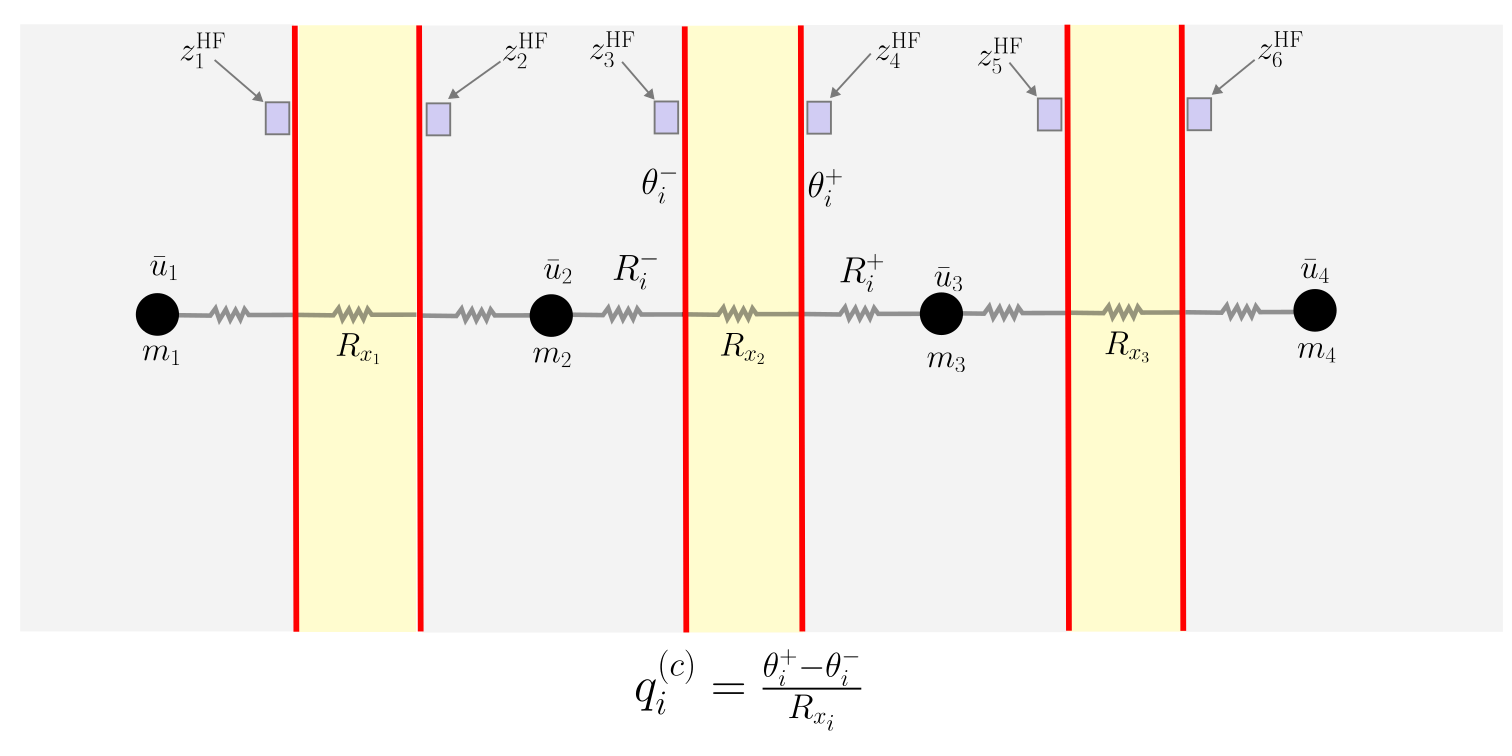
\includegraphics[width=0.9\textwidth]{./experiment.png}
\end{figure}
